\documentclass[12pt]{article}
\usepackage[italian]{babel}
\usepackage{amsmath}
\usepackage{siunitx}
\usepackage{derivative}
\usepackage{graphicx}
\usepackage[a4paper, total={6in, 9in}]{geometry}
\usepackage{caption}
\usepackage{subcaption}
\usepackage{float}

\title{Sviluppo e caratterizzazione di un amplificatore RF per rivelatori criogenici}
\author{Nicolas Bigiotti\\{\small Matr. 865437}\\{\small Cell. 3452438264 }\\[0.5cm]{\small Relatore: Claudio Gotti}\\{\small Correlatore: Gianluigi Ezio Pessina, Paolo Carniti}}

\date{19-20 Luglio 2023 - Corso di Laurea triennale in Fisica}


\begin{document}
\maketitle

Questa tesi si pone come obiettivo la realizzazione di un amplificatore in radiofrequenza (RF) con transistor bipolari a eterogiunzione SiGe e la successiva caratterizzazione a bassa temperatura. Amplificatori di questo tipo sono richiesti in molti ambiti sia di ricerca che industriali. Lo studio dei dispositivi a microonde è reso complesso dalle piccole lunghezze d'onda dei segnali coinvolti, comparabili con le dimensioni fisiche dei componenti circuitali. Inoltre prevedere e studiare il comportamento a temperature molto inferiori a quelle di normale esercizio non è banale data la mancanza di documentazione ufficiale sul transistor.

La prima fase di progettazione ha riguardato la scelta del punto di lavoro del transistor (Infineon BFP640). Per garantire una bassa potenza dissipata dal transistor durante l'esercizio è stata scelta una corrente di collettore $I_{C}=\SI{8}{\milli\ampere}$ e una tensione collettore-emettitore $V_{CE}=\SI{3.0}{\volt}$, individuato il punto di lavoro è stato possibile dedicarsi alla progettazione della parte di segnale.

Un tipico amplificatore RF è composto da una rete di adattamento di ingresso con il compito di adattare l'impedenza del generatore a quella in ingresso del transistor, una rete di adattamento di uscita per adattare l'impedenza d'uscita del transistor all'impedenza di carico e infine il transistor stesso, che fornisce l'amplificazione. A differenza di quanto accade a bassa frequenza per studiare la risposta di piccolo segnale non viene utilizzato un modello a componenti concentrati del transistor ma è necessario considerare i parametri di scattering che descrivono trasmissione e riflessione dei segnali elettrici all'ingresso e uscita del transistor. Per una tipica configurazione a emettitore comune, come quella usata in questo lavoro, i parametri sono forniti dal costruttore del transistor e possono essere utilizzati in simulazione per dimensionare le reti di ingresso e uscita.

Il primo passaggio di progettazione consiste nel valutare la stabilità della configurazione. Non trattandosi di un amplificatore reazionato tutta la potenziale instabilità è intrisecamente legata ai parametri di scattering del transistor che dipendono dalla frequenza di esercizio e dal punto di lavoro. In questo caso considerando un amplificatore a banda stretta centrata a $\SI{5}{\giga\hertz}$ il transistor risulta incodizionatamente stabile, vale a dire che indipendentemente dalle riflessioni introdotte dalle reti di adattamento l'amplificatore risulterà stabile e si ha piena libertà di progettazione di quest'ultime.

Garantita la stabilità si procede progettando le reti di adattamento in modo che venga garantito massimo trasferimento di potenza tra ingresso e uscita alla frequenza di esercizio. Per la realizzazione è stata utilizzata la tecnica a stub singolo che utilizza segmenti di linea di trasmissione opportunamente dimensionati per ottenere l'adattamento di impedenza voluto.
Una volta definito lo schema elettrico è stata realizzata la scheda con il software open source KiCad in modo da rendere possibile la produzione del circuito stampato da una ditta specializzata. Una volta ricevuta la scheda, i componenti precedentemente selezionati e acquistati sono stati saldati.

Con l'ausilio di un analizzatore vettoriale di rete è stata fatta una misura completa dei parametri di scattering a temperatura ambiente, osservando un buon accordo con i valori previsti in fase di progetto. Alla frequenza di interesse $\SI{5}{\giga\hertz}$ le impedenze di ingresso e uscita sono molto vicine a $\SI{50}{\ohm}$, e il guadagno è pari a $\SI{12}{\decibel}$. Inoltre è stato possibile verificare la funzionalità dell'amplificatore osservando nel dominio del tempo il segnale di uscita in presenza di una sinusoide in ingresso. Le misure sono state ripetute a temperatura criogenica fino a $\SI{4}{\kelvin}$. L'amplificatore è rimasto funzionante lungo tutto il processo di raffreddamento. Misure dei parametri di scattering hanno messo in evidenza l'efficacia delle reti di adattamento anche a bassa temperatura, mentre si è osservata una diminuzione del guadagno del transistor
\begin{figure}[H]
    \centering
    \begin{subfigure}[t]{0.45\textwidth}
        \centering
        \includegraphics[width=\textwidth]{img/IMG_2169.jpg}
        \caption{La scheda completa dopo la saldatura e il montaggio nell'involucro metallico necessario per un buon contatto termico con il criostato}
    \end{subfigure}
    \hfill
    \begin{subfigure}[t]{0.45\textwidth}
        \centering
        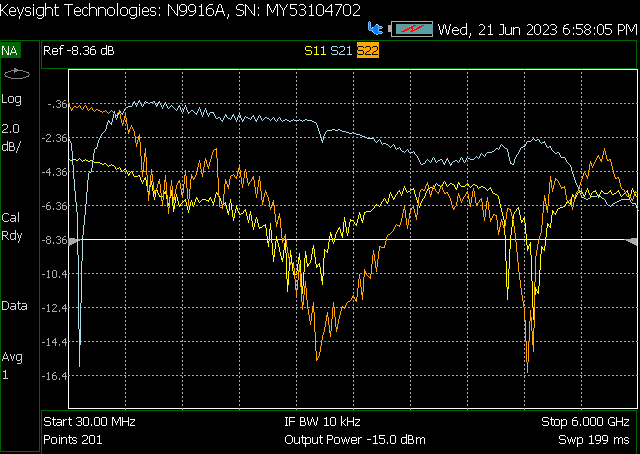
\includegraphics[width=\textwidth]{img/STUB_NO_COP.png}
        \caption{Parametri di scattering $S_{11}$, $S_{22}$, $S_{12}$ e $S_{21}$ misurati a temperatura ambiente (IMMAGINE DA RIFARE CON VNA BELLO INCLUDENDO ANCHE S12)}
    \end{subfigure}
\end{figure}



\end{document}